\documentclass{article}
\usepackage{graphicx} % Required for inserting images
\usepackage{subcaption}
\usepackage{listings}
\usepackage{amsmath, amssymb, booktabs}
\usepackage{hyperref}
\usepackage{listings}
\usepackage{comment}
\graphicspath{ {./figures/} }
\usepackage{xcolor}  % Required for color customization
\hypersetup{
  colorlinks=true,  % Activates colored links
  linkcolor=blue,   % Color of internal links (sections, pages, etc.)
  citecolor=blue,   % Color of citation links
  urlcolor=blue     % Color of external links (URLs)
}


\title {CAT Got Your Tongue? \\
\large Stock Returns Forecasting Using ARMA-GARCH}
\author{Johnathan Ferdinand, Devina Gera, Archimedes Li, Henry Liu, \\Katherine Shi, Sam Stevens}
\date{\today}
\begin{document}
\maketitle

\section{Introduction}
The ARMA-GARCH model is a model used to analyze time series data exhibiting both autocorrelation in its mean and time-varying volatility.  The ARMA component models the conditional mean as dependent on past values and errors, while the GARCH component models volatility by using the conditional variance as dependent on past squared errors and past variances.

\noindent We use this model to forecast the stock price CAT, a construction company.  The ARMA-GARCH model is especially useful for modelling stocks because stock prices often are correlated with their prices at past time steps.  The volatility of stocks often occurs in “bursts,” where time steps of high variance are seen close to other time steps of high variance.

\noindent The R packages we used were quantmod, lmtest, dplyr, PerformanceAnalytics, ggplot2, xts, tidyverse, “feasts”, “fable”, “lubridate”, “gridExtra”, tseries, forecast, and rugarch. 

\noindent Our results include forecasting returns over the period of June 1, 2017 to May 1, 2021 and comparing our predicted returns to the actual returns over this time period. 

\section{Data Description}
\noindent For our data, we used historical stock prices for Caterpillar (ticker: CAT) ranging from March 13, 1986 to May 31, 2017 for our training and from June 1, 2017 to May 1, 2021 for our testing data, gathered daily. The data was gathered from the Yahoo finance source built into R, and all data points were gathered on the daily timeframe. 

\noindent For each day, we stored two values: the price of the stock and the returns of the stock (relative to the price at the start date).

\noindent We did not remove any outliers, as for our task of forecasting stock returns, outliers in return or prices typically have underlying macroeconomic causes such as earnings calls, and removing these points would make it difficult to forecast such shifts in price in the future.


\section{Analysis}
We can see that the price increases over time despite showing volitility. The mean and variance change over time so the stock price is not stationary. (Figure \ref{fig:stockPrices}).

\noindent We then ran the Augmented Dickey-Fuller test on the data and got the following output:
\begin{verbatim}
Dickey-Fuller = -3.1858, Lag order = 19, p-value = 0.09026
alternative hypothesis: stationary
\end{verbatim}
We get a P value of $0.09$, thus we fail to reject the null hypothesis, and the Price of the stock is non-stationary.


\noindent Figure \ref{fig:return} gives that the average return on CAT is $0$. At a quick glance, we can see that the mean is approximately 0 (fig \ref{fig:return}\subref{fig:returnCat}). The histogram showing a normal distribution with mean 0 confirms our suspicions (fig \ref{fig:return}\subref{fig:returnHisto}).

\noindent We ran the same test again for the return of the stock and got the following output:
\begin{verbatim}
Dickey-Fuller = -20.102, Lag order = 19, p-value = 0.01
alternative hypothesis: stationary
\end{verbatim}
This time, we reject the null hypothesis, so the return on the stocks is non-stationary.

\noindent The ACF shows that the return series is not dependent on the previous day's error.
          The PACF shows that the return series autocorrelates with lags.
	  Thus, the Return series are influenced by previous days Return.(Figure \ref{fig:acf})

	  \noindent The absence of autocorrelation is confirmed by the Box-Ljung test, which gives an output of 
	  \begin{verbatim}
	  X-squared = 7.3365, df = 1, p-value = 0.006757
	  \end{verbatim}
We reject the null hypothesis,  thus the return series is not independent.

\noindent The plot of ACF of square return values (Fig \ref{fig:acfErr}) shows a clear but slow decay of auto correlation.

\noindent The rolling performance chart points to GARMA being able to improve our ARMA model. (Fig \ref{fig:volatility})

\noindent The output from our best GARCH model is the following
\clearpage
\begin{verbatim}
*---------------------------------*
*          GARCH Model Fit        *
*---------------------------------*

Conditional Variance Dynamics 	
-----------------------------------
GARCH Model	: eGARCH(2,1)
Mean Model	: ARFIMA(1,0,1)
Distribution	: std 

Optimal Parameters
------------------------------------
        Estimate  Std. Error     t value Pr(>|t|)
mu      0.000261    0.000177  1.4722e+00 0.140969
ar1    -0.102506    0.095543 -1.0729e+00 0.283324
ma1     0.144743    0.094731  1.5279e+00 0.126528
omega  -0.051581    0.000756 -6.8242e+01 0.000000
alpha1 -0.034245    0.019206 -1.7831e+00 0.074577
alpha2 -0.001064    0.019053 -5.5863e-02 0.955451
beta1   0.993576    0.000057  1.7412e+04 0.000000
gamma1  0.196479    0.024228  8.1095e+00 0.000000
gamma2 -0.116456    0.018339 -6.3501e+00 0.000000
shape   5.466915    0.307001  1.7807e+01 0.000000

Robust Standard Errors:
        Estimate  Std. Error     t value Pr(>|t|)
mu      0.000261    0.000171  1.5240e+00 0.127512
ar1    -0.102506    0.035790 -2.8641e+00 0.004182
ma1     0.144743    0.035388  4.0901e+00 0.000043
omega  -0.051581    0.000978 -5.2729e+01 0.000000
alpha1 -0.034245    0.021049 -1.6269e+00 0.103752
alpha2 -0.001064    0.020370 -5.2253e-02 0.958327
beta1   0.993576    0.000068  1.4595e+04 0.000000
gamma1  0.196479    0.027597  7.1196e+00 0.000000
gamma2 -0.116456    0.022591 -5.1549e+00 0.000000
shape   5.466915    0.343479  1.5916e+01 0.000000

LogLikelihood : 20632.85 

Information Criteria
------------------------------------
                    
Akaike       -5.2422
Bayes        -5.2333
Shibata      -5.2422
Hannan-Quinn -5.2392

Weighted Ljung-Box Test on Standardized Residuals
------------------------------------
                        statistic p-value
Lag[1]                     0.3717  0.5421
Lag[2*(p+q)+(p+q)-1][5]    0.9673  1.0000
Lag[4*(p+q)+(p+q)-1][9]    2.7815  0.9210
d.o.f=2
H0 : No serial correlation

Weighted Ljung-Box Test on Standardized Squared Residuals
------------------------------------
                         statistic p-value
Lag[1]                       3.030 0.08172
Lag[2*(p+q)+(p+q)-1][8]      6.991 0.15192
Lag[4*(p+q)+(p+q)-1][14]     8.895 0.29087
d.o.f=3

Weighted ARCH LM Tests
------------------------------------
            Statistic Shape Scale P-Value
ARCH Lag[4]    0.1471 0.500 2.000  0.7014
ARCH Lag[6]    1.2888 1.461 1.711  0.6667
ARCH Lag[8]    2.2547 2.368 1.583  0.6900

Nyblom stability test
------------------------------------
Joint Statistic:  4.313
Individual Statistics:             
mu     0.2269
ar1    1.0315
ma1    0.9868
omega  0.3838
alpha1 0.9470
alpha2 1.1558
beta1  0.3848
gamma1 0.1460
gamma2 0.3022
shape  0.4216

Asymptotic Critical Values (10% 5% 1%)
Joint Statistic:     	 2.29 2.54 3.05
Individual Statistic:	 0.35 0.47 0.75

Sign Bias Test
------------------------------------
                   t-value   prob sig
Sign Bias           1.5380 0.1241    
Negative Sign Bias  1.4312 0.1524    
Positive Sign Bias  0.8153 0.4149    
Joint Effect        3.0811 0.3793    


Adjusted Pearson Goodness-of-Fit Test:
------------------------------------
  group statistic p-value(g-1)
1    20     16.89       0.5976
2    30     39.82       0.0869
3    40     42.79       0.3118
4    50     54.50       0.2734
\end{verbatim}

\noindent We can see from the Ljung-Box test that there is no evidence of serial correlation or remaining ARCH effects. \\

\noindent From the ARCH LM test, we can see that there are no remaining ARCH effects

\noindent The model also converges and has a persistence of Volatility of $0.9936$.

\noindent The plots for out model are in figure \ref{fig:garch}.

\clearpage

\begin{figure}[h]
	\centering
	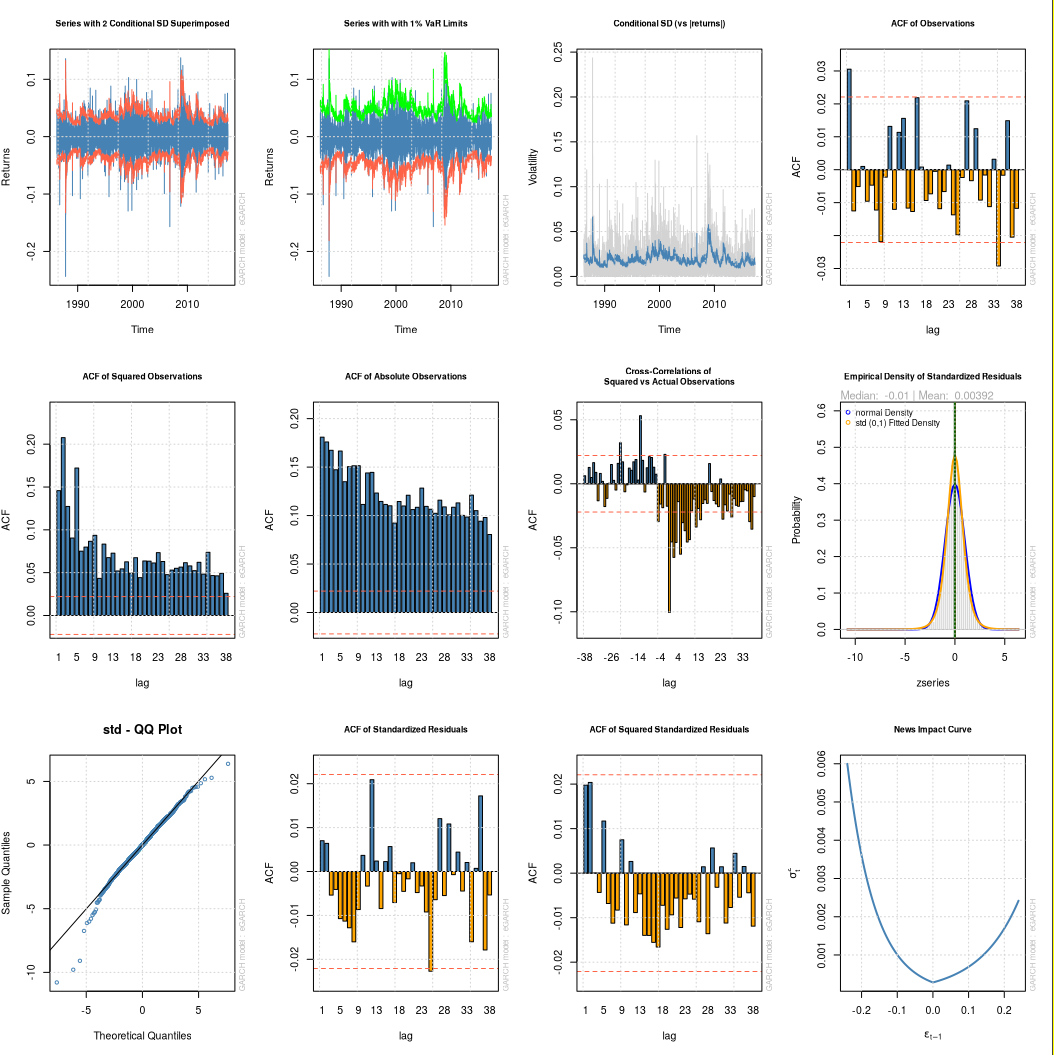
\includegraphics[width=\linewidth]{garch}
	\caption{Plots for the selected model.}
	\label{fig:garch}
\end{figure}

\begin{figure}[h]
	\centering
	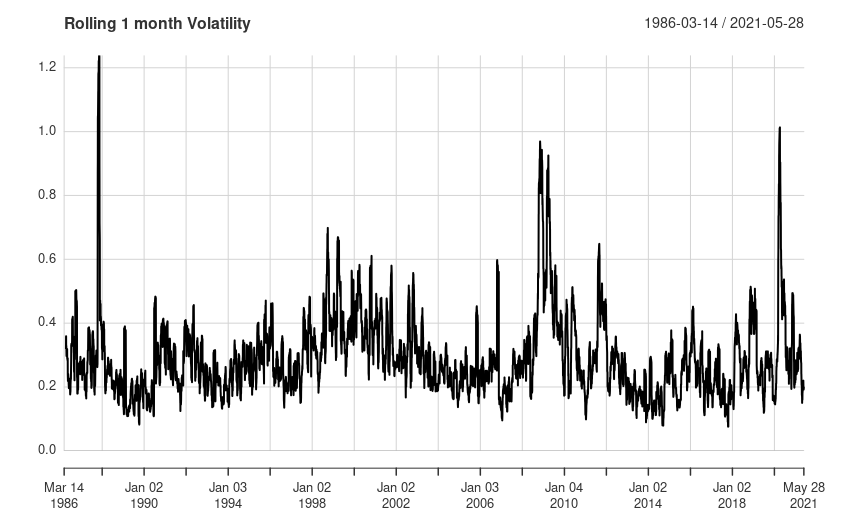
\includegraphics[width=\linewidth]{monthly_volatility}
	\caption{Rolling 1 month volatility for CAT.}
	\label{fig:volatility}
\end{figure}
\begin{figure}[h]
	\centering
	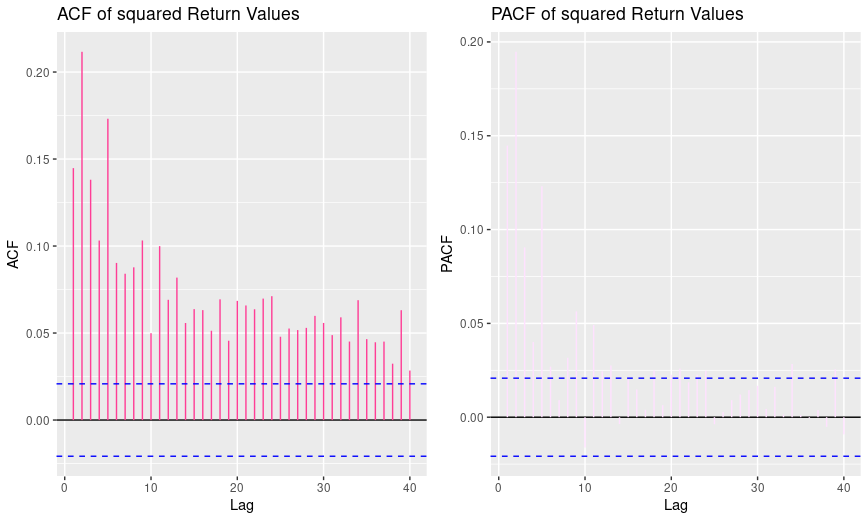
\includegraphics[width=\linewidth]{acf_pacf_squared}
	\caption{ACF of return values (left) and PACF of return values(right)}
	\label{fig:acfErr}
\end{figure}

\begin{figure}[h]
	\centering
	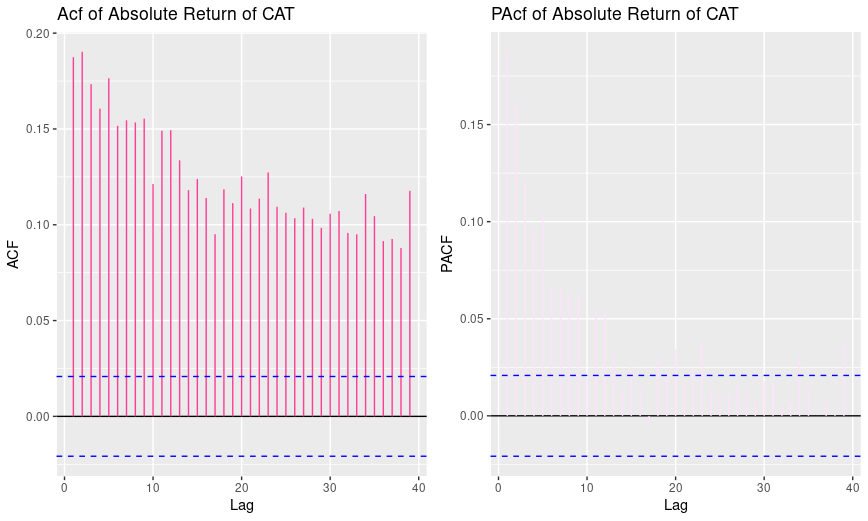
\includegraphics[width=\linewidth]{acf_pacf_of_cat}
	\caption{ACF of return values (left) and PACF of return values(right)}
	\label{fig:acf}
\end{figure}

\begin{figure}[h]
	\centering
	\begin{subfigure}{\linewidth}
		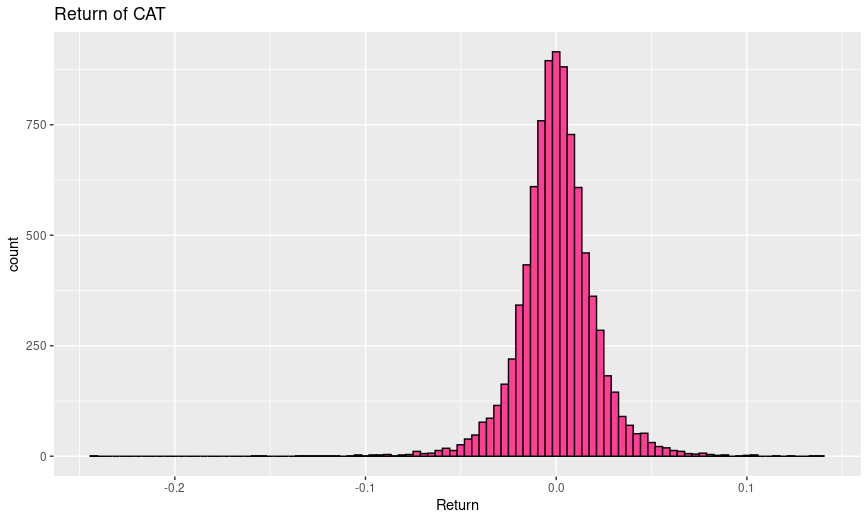
\includegraphics[width=\linewidth]{return_of_cat_histo}
		\caption{Histogram for fig \ref{fig:returnCat}}
		\label{fig:returnHisto}
	\end{subfigure}
	\centering
	\begin{subfigure}{\linewidth}
		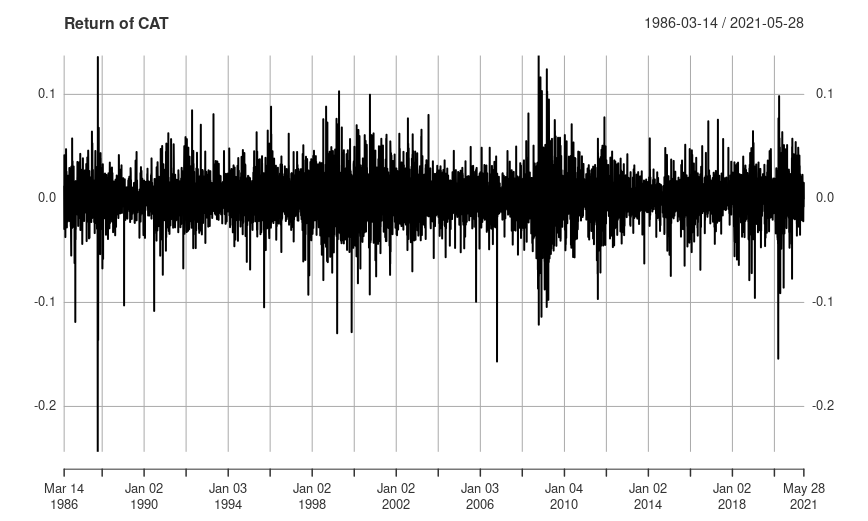
\includegraphics[width=\linewidth]{return_of_cat}
		\caption{Return of CAT as a function of time, at monthly intervals}
		\label{fig:returnCat}
	\end{subfigure}
	\caption{The returns of CAT over time.}
	\label{fig:return}
\end{figure}

\begin{figure}[h]
	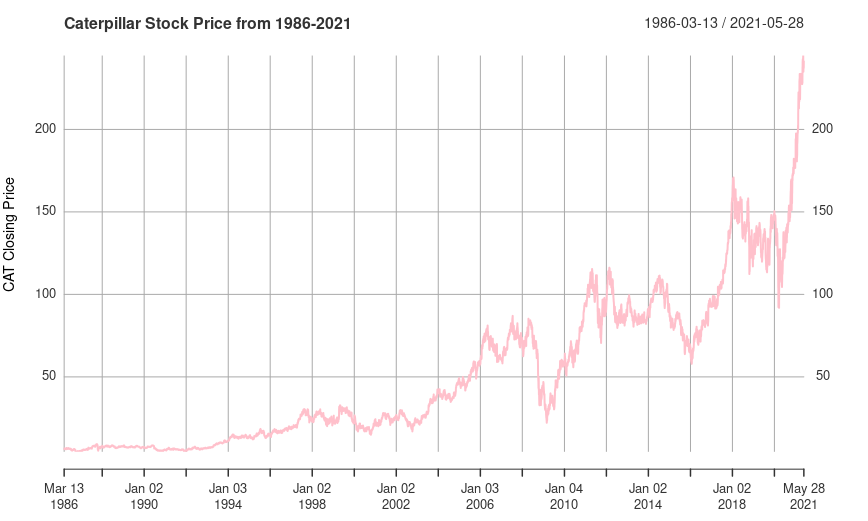
\includegraphics[width=\linewidth]{caterpillar_stock_price}
	\caption{The stock price of caterpillar as a function of time from 1986 - 2021}
	\label{fig:stockPrices}
\end{figure}
\clearpage

\section{Model Evaluation and Prediction}
We evaluated several ARMA-GARCH models to determine the best fit for forecasting Caterpillar (CAT) stock returns and then use it for prediction.

We fit eight candidate models combining ARMA structures with eGARCH (exponential GARCH) volatility components. Specifically, we tested:
\begin{itemize}
	\item ARMA(0,0)-eGARCH(1,1)
	\item ARMA(1,1)-eGARCH(1,1
	\item ARMA(2,2)-eGARCH(1,1)
	\item ARMA(0,0)-eGARCH(1,2)
	\item ARMA(1,1)-eGARCH(2,1)
	\item ARMA(3,1)-eGARCH(1,1)
	\item ARMA(3,2)-eGARCH(1,1)
	\item ARMA(1,3)-eGARCH(1,1)
\end{itemize}

We evaluated the models using the Akaike Information Criterion (AIC), which balances model fit with complexity, a lower AIC indicates a better model. The AIC results were:
\begin{verbatim}
Model
AIC
fit_garch_1 (ARMA(0,0)-eGARCH(1,1))
-5.2411 
fit_garch_2 (ARMA(1,1)-eGARCH(1,1))
-5.2414
fit_garch_3 (ARMA(2,2)-eGARCH(1,1))
-5.2422
fit_garch_4 (ARMA(0,0)-eGARCH(1,2))
 -5.2419
fit_garch_5 (ARMA(1,1)-eGARCH(2,1))
-5.2427
fit_garch_6 (ARMA(3,1)-eGARCH(1,1))
-5.2422
fit_garch_7 (ARMA(3,2)-eGARCH(1,1))
-5.2420
fit_garch_8 (ARMA(1,3)-eGARCH(1,1))
-5.2422
\end{verbatim}

We found that \texttt{fit\_garch\_5 (ARMA(1,1)-eGARCH(2,1))} provided the best balance of fit and simplicity, as it achieved the lowest AIC among the tested models.

Further to prove the efficiency of the model we also check for after subset selection:

\begin{itemize}
	\item Model summary: The ARMA(1,1) component captures short-term dependencies in the return series, while the eGARCH(2,1) component models asymmetric volatility effects (such as the leverage effect, where negative shocks impact volatility differently from positive shocks).


\item Persistence of volatility: We measured how much past volatility carries into future volatility. A high persistence value suggests the presence of volatility clustering, a common feature in financial time series.


\item Model convergence: We verified that the model estimation converged successfully, confirming that the parameter estimates are stable and reliable.
\end{itemize}


 We then used the final model for forecasting the returns and price data for the period from June 1, 2017 to May 1, 2021:

 \begin{itemize}
	 \item Static 50-day ahead forecast: We predicted the next 50 days of returns and volatility, providing both expected future returns and confidence intervals. We found a mean error of 0.00039 and an RMSE of 0.0208.


	 \item Rolling forecast: We implemented a rolling window approach to simulate dynamic updating over time, showing how the model would perform in a live forecasting setting. We found a mean error of 0.0004 and an RMSE of 0.02.


	 \item Bootstrap forecast: We generated bootstrapped forecasts which produced a distribution of possible future paths to account for estimation uncertainty, offering a more robust prediction framework.
\end{itemize}

From this, using the Box-Ljung test, we found no autocorrelation in the errors, finding a $X^2$ value of $173$ on the rolling forecast errors with a p-value < $2.2e-16$. 

 To assess the model’s accuracy and suitability, we used:
 \begin{itemize}
\item AIC for in-sample fit comparison.


\item Residual diagnostics (including plots and the Ljung-Box test) to ensure no remaining autocorrelation or heteroskedasticity in the residuals.


\item Forecast plots comparing predicted vs. actual returns to visually evaluate performance.
\end{itemize}


In summary, the ARMA(1,1)-eGARCH(2,1) model was selected as the final model based on thorough assessment

\section{Conclusion}
Our chosen model performed quite poorly in the immediate future despite having a low MSE of 0.00039 for the 50-day ahead forecast.  The reason this MSE is so small is because the scale of the CAT stock price is small.  If we look at the forecast predictions compared to the true stock prices, it captures very little of the volatility shown in the plot.  In consolation, the forecast does show some ups and downs that do line up with the true trends.

\begin{figure}[h]
	\centering
	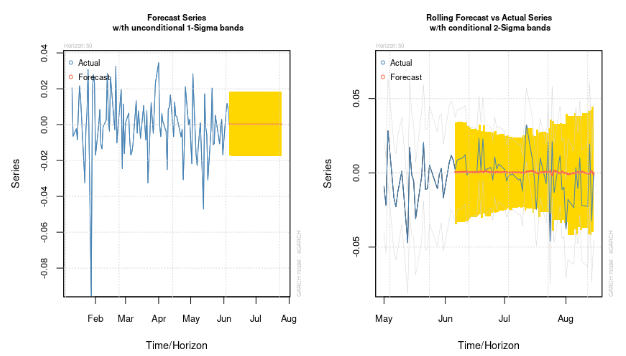
\includegraphics[width=0.9\linewidth]{forecast.png}
	\caption{Forcast Series and Rolling Forecast with sigma bands}
	\label{fig:forecast-series}
\end{figure}

\section{Appendix A: Code}
\href{https://github.com/mshki/math-456/blob/main/essay_6/main.R}{Here,} or below:
\begin{verbatim}
# 0 Import Libraries
library("Cairo")
library(quantmod) # for quantitative financial modeling and testing
library(lmtest) # For diagnostic checking in linear regression models
library(dplyr) # For wrking with data frame 
library(PerformanceAnalytics) # For portfolio performance and analysis
library(ggplot2) # For plots
library(xts) # For extensible time series
library(tidyverse) # For data visualization 
library("feasts") # For "Feature Extraction And Statistics for Time Series" 
library("fable") # FOr commonly used time series forecasting models
library("lubridate") # For working with date-times and time-spans
library("gridExtra") # For grids
library(tseries) # For  time series analysis and computational finance
library(forecast) # For analyzing forecasts 
library(rugarch) # For univariate GARCH models

# 1 Get Data
getSymbols("CAT", src="yahoo", periodicity = "daily", from = "1986-03-13", to = "2017-05-31")
head(CAT)

# 2 Calculate (log) returns
data <- cbind(
  Price = CAT$CAT.Close,
  Return=CalculateReturns(CAT$CAT.Close, method = 'log')) 
colnames(data) <- c('Price','Return')
head(data)

# 3 Verify Assumptions
plot(na.omit(data$Price), ylab='CAT Closing Price',main='Caterpillar Stock Price from 1986-2017',col='pink')
# Observe: The price increases over time despite showing volatility 
#          Mean and variance change over time.
#          Thus, stock price is NOT stationary over time

plot(na.omit(data$Return),main='Return of CAT')
# Observe: The stock's returns' mean and variance are constant overtime 
#          Thus, stock returns are stationary over time

# 3.1 Augmented Dickey Fuller Test (Stationary Test)
#     Checking whether Price is Stationary 
adf.test(na.omit(data$Price))
# Observe: p-value = 0.99 > alpha = 0.05
#          We fail to reject null hypothesis 
#          Thus, Price of stock is not stationary

#      Checking whether Return is Stationary 
adf.test(na.omit(data$Return))
# Observe: p-value = 0.01 < alpha = 0.05
#          We reject null hypothesis 
#          Thus, Return of stock is stationary

# 3.2 (Partial) Autocorrelation Function
#      Checking whether Return is Autocorrelated
acf(na.omit(data$Return), lag.max = 40, main='ACF of Return Values',col='violetred1')
pacf(na.omit(data$Return), main='Partial Auto Correlation of Return Values',col='violetred1')
# Observe: ACF shows Return series is not dependent on previous days error
#          PACF shows Return series autocorrelates with lags 
#          Thus, Return series are influenced by previous days Return

# 3.3 Normality Test 
ggplot(aes(Return), data=data) + geom_histogram(bins = 100,col='black',fill='violetred1') + ggtitle('Return of CAT')
skewness(data$Return); kurtosis(data$Return)
# Observe: Returns are not normally distributed!
#          Negative skew indicates Leptokurtic distribution

skewness(data$Return); kurtosis(data$Return)
# Observe: QQ Plot Verifies distribution of Returns 

jarque.bera.test(na.omit(data$Return))
# Observe: Jarque Bera Test 
#          p-value < 2.2e-16 < alpha = 0.05
#          We reject null hypothesis 
#          Thus Return series is not normally distributed

# 3.4 Absence of Auto Correlation
Box.test(na.omit(data$Return), type = "Ljung-Box")
# Observe: Ljung-Box Test 
#          p-value < 0.05751 < alpha = 0.01
#          We reject null hypothesis 
#          Thus Return series is not independent

# 3.5 Autocorrelation of Absolute/Squaare Return
a<- ggAcf(abs(na.omit(data$Return)), col='violetred1',main='Acf of Absolute Return of CAT')
p<- ggPacf(abs(na.omit(data$Return)),col='thistle1',main='PAcf of Absolute Return of CAT')
grid.arrange(a,p, ncol = 2, nrow = 1)
# Observe: Absolute Return series show slow decay of auto correlation 

c <- ggAcf(na.omit(data$Return)^2, lag.max = 40, col='violetred1', main='ACF of squared Return Values')
d<- ggPacf(na.omit(data$Return)^2,lag.max = 40, col='thistle1',main= 'PACF of squared Return Values')
grid.arrange(c,d, ncol = 2, nrow = 1)
# Observe: Squared Return series show slow decay of auto correlation 

# 3.6 Volatility Clustering 
chart.RollingPerformance(na.omit(data$Return),width = 22,FUN = 'sd.annualized',scale=252, main = 'Rolling 1 month Volatility')
# Observe: We can significantly improve our ARMA model using GARCH 

# 4 Fit the GARCH Model

#      Model 1: Fit ARMA(0,0)-gjrGARCH(1,1) model with Student t-distribution
CAT_garch_1 <- ugarchspec(mean.model =
                            list(armaOrder=c(0,0)),variance.model = list(model = 'eGARCH', garchOrder = c(1, 1)),distribution = 'std')
fit_garch_1 <- ugarchfit(spec = CAT_garch_1, data= na.omit(data$Return))
aic_1 <- infocriteria(fit_garch_1)[1]
fit_garch_1
#plot(fit_garch_1,which='all')

#      Model 2: Fit ARMA(1,1)-gjrGARCH(1,1) model with Student t-distribution
CAT_garch_2 <- ugarchspec(mean.model = list(armaOrder=c(1,1)),variance.model = list(model = 'eGARCH', garchOrder = c(1, 1)),distribution = 'std')
fit_garch_2 <- ugarchfit(spec = CAT_garch_2, data= na.omit(data$Return))
aic_2 <- infocriteria(fit_garch_2)[1]
aic_2
fit_garch_2
#plot(fit_garch_2,which='all')

#      Model 3: Fit ARMA(2,2)-gjrGARCH(1,1) model with Student t-distribution
CAT_garch_3 <- ugarchspec(mean.model = list(armaOrder=c(2,2)),variance.model = list(model = 'eGARCH', garchOrder = c(1, 1)),distribution = 'std')
fit_garch_3 <- ugarchfit(spec = CAT_garch_3, data= na.omit(data$Return))
aic_3 <- infocriteria(fit_garch_3)[1]
fit_garch_3
#plot(fit_garch_3,which='all')

#      Model 4: Fit ARMA(0,0)-eGARCH(1,2) model with Student t-distribution
CAT_garch_4 <- ugarchspec(mean.model = list(armaOrder=c(0,0)),variance.model = list(model = 'eGARCH', garchOrder = c(1, 2)),distribution = 'std')
fit_garch_4 <- ugarchfit(spec = CAT_garch_4, data= na.omit(data$Return))
aic_4 <- infocriteria(fit_garch_4)[1]
fit_garch_4
#plot(fit_garch_4,which='all')

#      Model 5: Fit ARMA(1,1)-eGARCH(2,1) model with Student t-distribution
CAT_garch_5 <- ugarchspec(mean.model = list(armaOrder=c(1,1)),variance.model = list(model = 'eGARCH', garchOrder = c(2,1)),distribution = 'std')
fit_garch_5 <- ugarchfit(spec = CAT_garch_5, data= na.omit(data$Return))
aic_5 <- infocriteria(fit_garch_5)[1]
fit_garch_5
#plot(fit_garch_5,which='all')

#      Model 6: Fit ARMA(3,1)-eGARCH(1,1) model with Student t-distribution
CAT_garch_6 <- ugarchspec(mean.model = list(armaOrder=c(3,1)),variance.model = list(model = 'eGARCH', garchOrder = c(1, 1)),distribution = 'std')
fit_garch_6 <- ugarchfit(spec = CAT_garch_6, data= na.omit(data$Return))
aic_6 <- infocriteria(fit_garch_6)[1]
fit_garch_6
#plot(fit_garch_6,which='all')

#      Model 7: Fit ARMA(3,2)-eGARCH(1,1) model with Student t-distribution
CAT_garch_7 <- ugarchspec(mean.model = list(armaOrder=c(3,2)),variance.model = list(model = 'eGARCH', garchOrder = c(1, 1)),distribution = 'std')
fit_garch_7 <- ugarchfit(spec = CAT_garch_7, data= na.omit(data$Return))
aic_7 <- infocriteria(fit_garch_7)[1]
fit_garch_7
#plot(fit_garch_7,which='all')

#      Model 8: Fit ARMA(1,3)-eGARCH(1,1) model with Student t-distribution
CAT_garch_8 <- ugarchspec(mean.model = list(armaOrder=c(1,3)),variance.model = list(model = 'eGARCH', garchOrder = c(1, 1)),distribution = 'std')
fit_garch_8 <- ugarchfit(spec = CAT_garch_8, data= na.omit(data$Return))
aic_8 <- infocriteria(fit_garch_8)[1]
fit_garch_8
#plot(fit_garch_8,which='all')


# 5 Model Selection
Model = c('fit_garch_1','fit_garch_2','fit_garch_3','fit_garch_4','fit_garch_5','fit_
garch_6','fit_garch_7','fit_garch_8')
AIC = c(aic_1, aic_2, aic_3, aic_4, aic_5, aic_6, aic_7, aic_8)
(model <- data.frame(Model,AIC))
which.min(model[,'AIC'])
# Observe: The output was 5, so our selected model is fit_garch_5

# 6 Analyze Selected Model
#      Statistics & Plot
fit_garch_5
plot(fit_garch_5,which='all')   

#      Persistence of Volatility
persistence(fit_garch_5) 

#      Convergence of the Model
print(convergence(fit_garch_5))

# 7 Forecasting
test_start <- as.Date("2017-06-01")
test_end   <- as.Date("2021-05-01")

rets <- data$Return
test_rets  <- window(rets, start = test_start, end = test_end)
n.out <- length(test_rets)

forecast <-ugarchforecast(fit_garch_5,data=data,n.ahead=n.out)
forecast_ret <- as.numeric(forecast@forecast$seriesFor)
forecast

#      Rolling Forecast 
fit_roll <- ugarchfit(CAT_garch_5, data= na.omit(data$Return),out.sample =500)
fore_roll <- ugarchforecast(fit_roll, n.ahead=n.out, n.roll=50)
fore_roll_ret <- as.numeric(fore_roll@forecast$seriesFor)
fore_roll

par(mfrow=c(1,2))
plot(fore_roll,which=1)
plot(fore_roll,which=2)

#      Bootstrap Forecast
par(mfrow=c(1,2))
fore_boot <- ugarchboot(fit_garch_5,data = na.omit(data$Return), method = c("Partial", "Full")[1], n.ahead = n.out, n.bootpred = 500)
fore_boot_ret <- t(as.data.frame(fore_boot, which = "series", type = "summary"))
plot(fore_boot,which=2)
plot(fore_boot,which=3)

# 8 Model Evaluation
# 8.1 Forecast accuracy metrics: ME, RMSE, MAE, MPE, MAPE
acc_forecast <- accuracy(forecast_ret, as.numeric(test_rets))
acc_fore_roll <- accuracy(fore_roll_ret, as.numeric(test_rets))
#acc_fore_boot <- accuracy(fore_boot_ret, as.numeric(test_rets))

acc_forecast
acc_fore_roll
#acc_fore_boot

# 8.2 Test whether forecast errors have zero mean (t‑test)
#    – H: mean(error) = 0
fore_errors <- as.numeric(test_rets) - forecast_ret
t.test(fore_errors)
fore_roll_errors <- as.numeric(test_rets) - fore_roll_ret
t.test(fore_roll_errors)

# 8.3 Check for autocorrelation in errors (Ljung‑Box)
#    – H: no autocorrelation up to default lag
Box.test(fore_errors, type = "Ljung-Box")
Box.test(fore_roll_errors, type = "Ljung-Box")
\end{verbatim}

\end{document}
